% ============================================================
%  PROBLEM 2 — worked example
%  Shows: a \resizebox'd table, a side-by-side subfigure pair,
%         inline math and footnotes.
% ============================================================

\section*{Problem 2}
\phantomsection
\addcontentsline{toc}{section}{Problem 2}

The task is to describe the family of plane curves traced by two perpendicular
harmonic oscillations, and to determine when the resulting figure closes on
itself. The pair of parametric equations is

\begin{equation} \label{lissajous}
	x(t) = \sin(at + \delta) \; \; \; \text{, } \; \; \; y(t) = \sin(bt)
	\; \; \; \text{, } t \in [0, 2\pi]
\end{equation}

where $a$ and $b$ are the two angular frequencies and $\delta$ is the phase
offset between them. The curves of \cref{lissajous} are the Lissajous figures,
the shape an oscilloscope draws when one signal is fed to each deflection
axis.

The closure condition follows from requiring both components to return to
their starting values at the same time. Component $x$ has period
$2\pi/a$ and component $y$ has period $2\pi/b$, so the curve closes after a
time $T$ that is a common multiple of both:

\begin{equation} \label{closure}
	T = \frac{2\pi m}{a} = \frac{2\pi n}{b}
	\; \; \Rightarrow \; \;
	\frac{a}{b} = \frac{m}{n} \; \; \; \text{, } m, n \in \mathbb{N}
\end{equation}

\Cref{closure} says that the figure is closed exactly when the frequency ratio
is rational. For an irrational ratio the trajectory never repeats and
eventually fills the square $[-1,1]^2$ densely\footnote{Which is why the
picture on an oscilloscope drifts instead of standing still when the two
generators are not phase-locked: the ratio is only ever rational to within the
stability of the instruments.}. When it is rational and written in lowest
terms, $m$ and $n$ count the tangencies with the vertical and horizontal edges
of the bounding box, which is the usual way to read the ratio off the screen.
\Cref{tab:ratios} lists the small cases.

\begin{table}[htbp]
	\centering
	\caption{Frequency ratios of \cref{lissajous} in lowest terms, the number of
	edge tangencies each produces, and the shape seen at zero phase offset.}
	\label{tab:ratios}
	\resizebox{11cm}{!}{
		\begin{tabular}{|c|c|c|c|}
			\hline
			$a : b$ & Horizontal tangencies & Vertical tangencies & Shape at $\delta = 0$ \\ \hline
			$1 : 1$ & 1 & 1 & Straight line (degenerate ellipse) \\ \hline
			$2 : 1$ & 1 & 2 & Parabola-like arc, traced twice     \\ \hline
			$3 : 2$ & 2 & 3 & Three-lobed knot                    \\ \hline
			$4 : 3$ & 3 & 4 & Woven square                        \\ \hline
			$5 : 4$ & 4 & 5 & Dense lattice                       \\ \hline
		\end{tabular}
	}
\end{table}

The phase offset $\delta$ does not change the closure condition of
\cref{closure}, only the appearance: at $\delta = 0$ the curve degenerates into
its self-intersecting form, and as $\delta$ grows towards $\pi/2$ the lobes
open up. \Cref{fig:lissajous} shows nine ratios, each drawn at three phase
offsets.

A second curve makes the contrast with \cref{lissajous} clear. Fay's butterfly
curve \cite{fay1989} is given in polar form as

\begin{equation} \label{butterfly}
	r(\theta) = e^{\cos \theta} - 2\cos(4\theta) + \sin^5\!\left(\frac{\theta}{12}\right)
	\; \; \; \text{, } \theta \in [0, 24\pi] \; \; \text{,  \cite{fay1989}}
\end{equation}

The third term of \cref{butterfly} has period $24\pi$ in $\theta$ while the
first two have period $2\pi$, so the ratio of periods is $12$ — rational, and
the curve therefore closes, but only after twelve turns. Each turn is offset
slightly from the last, which is what produces the layered wings in
\cref{fig:butterfly} rather than a single retraced outline.

\begin{figure}[htbp]
	\centering
	\begin{subfigure}[b]{0.48\linewidth}
		\centering
		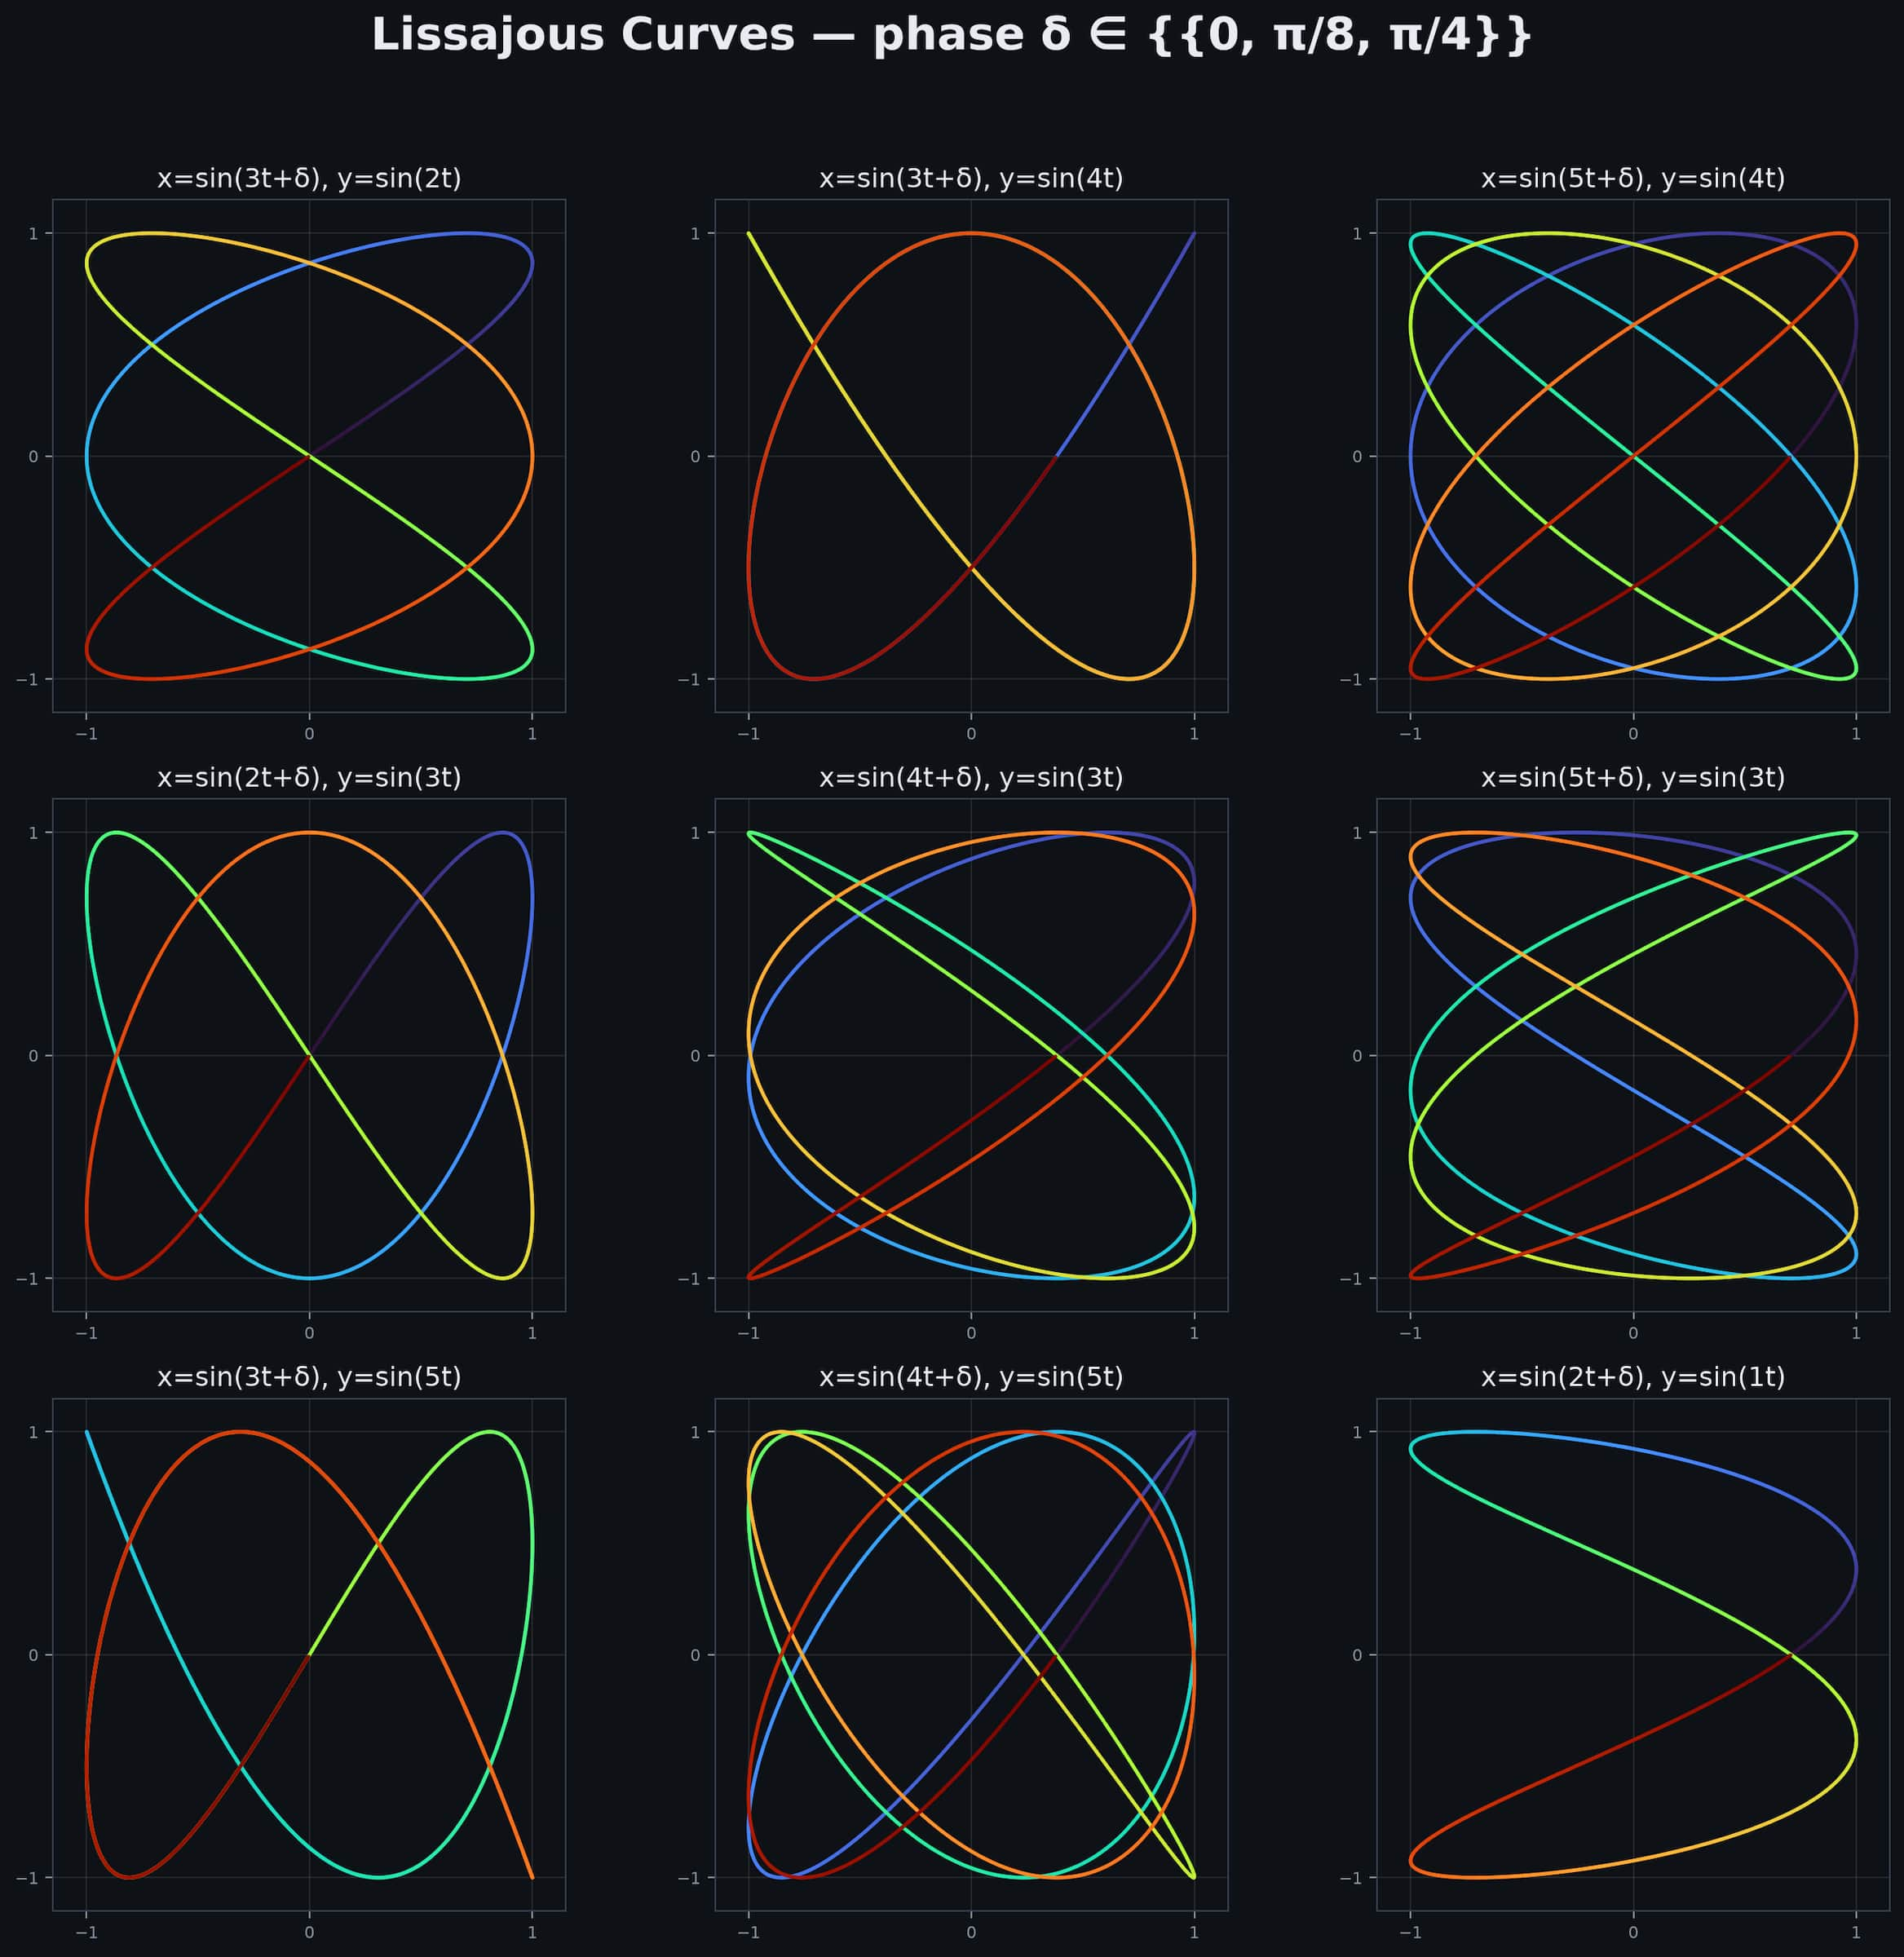
\includegraphics[width=\linewidth]{graphs/lissajous}
		\caption{Lissajous figures, \cref{lissajous}.}
		\label{fig:lissajous}
	\end{subfigure}
	\hfill
	\begin{subfigure}[b]{0.48\linewidth}
		\centering
		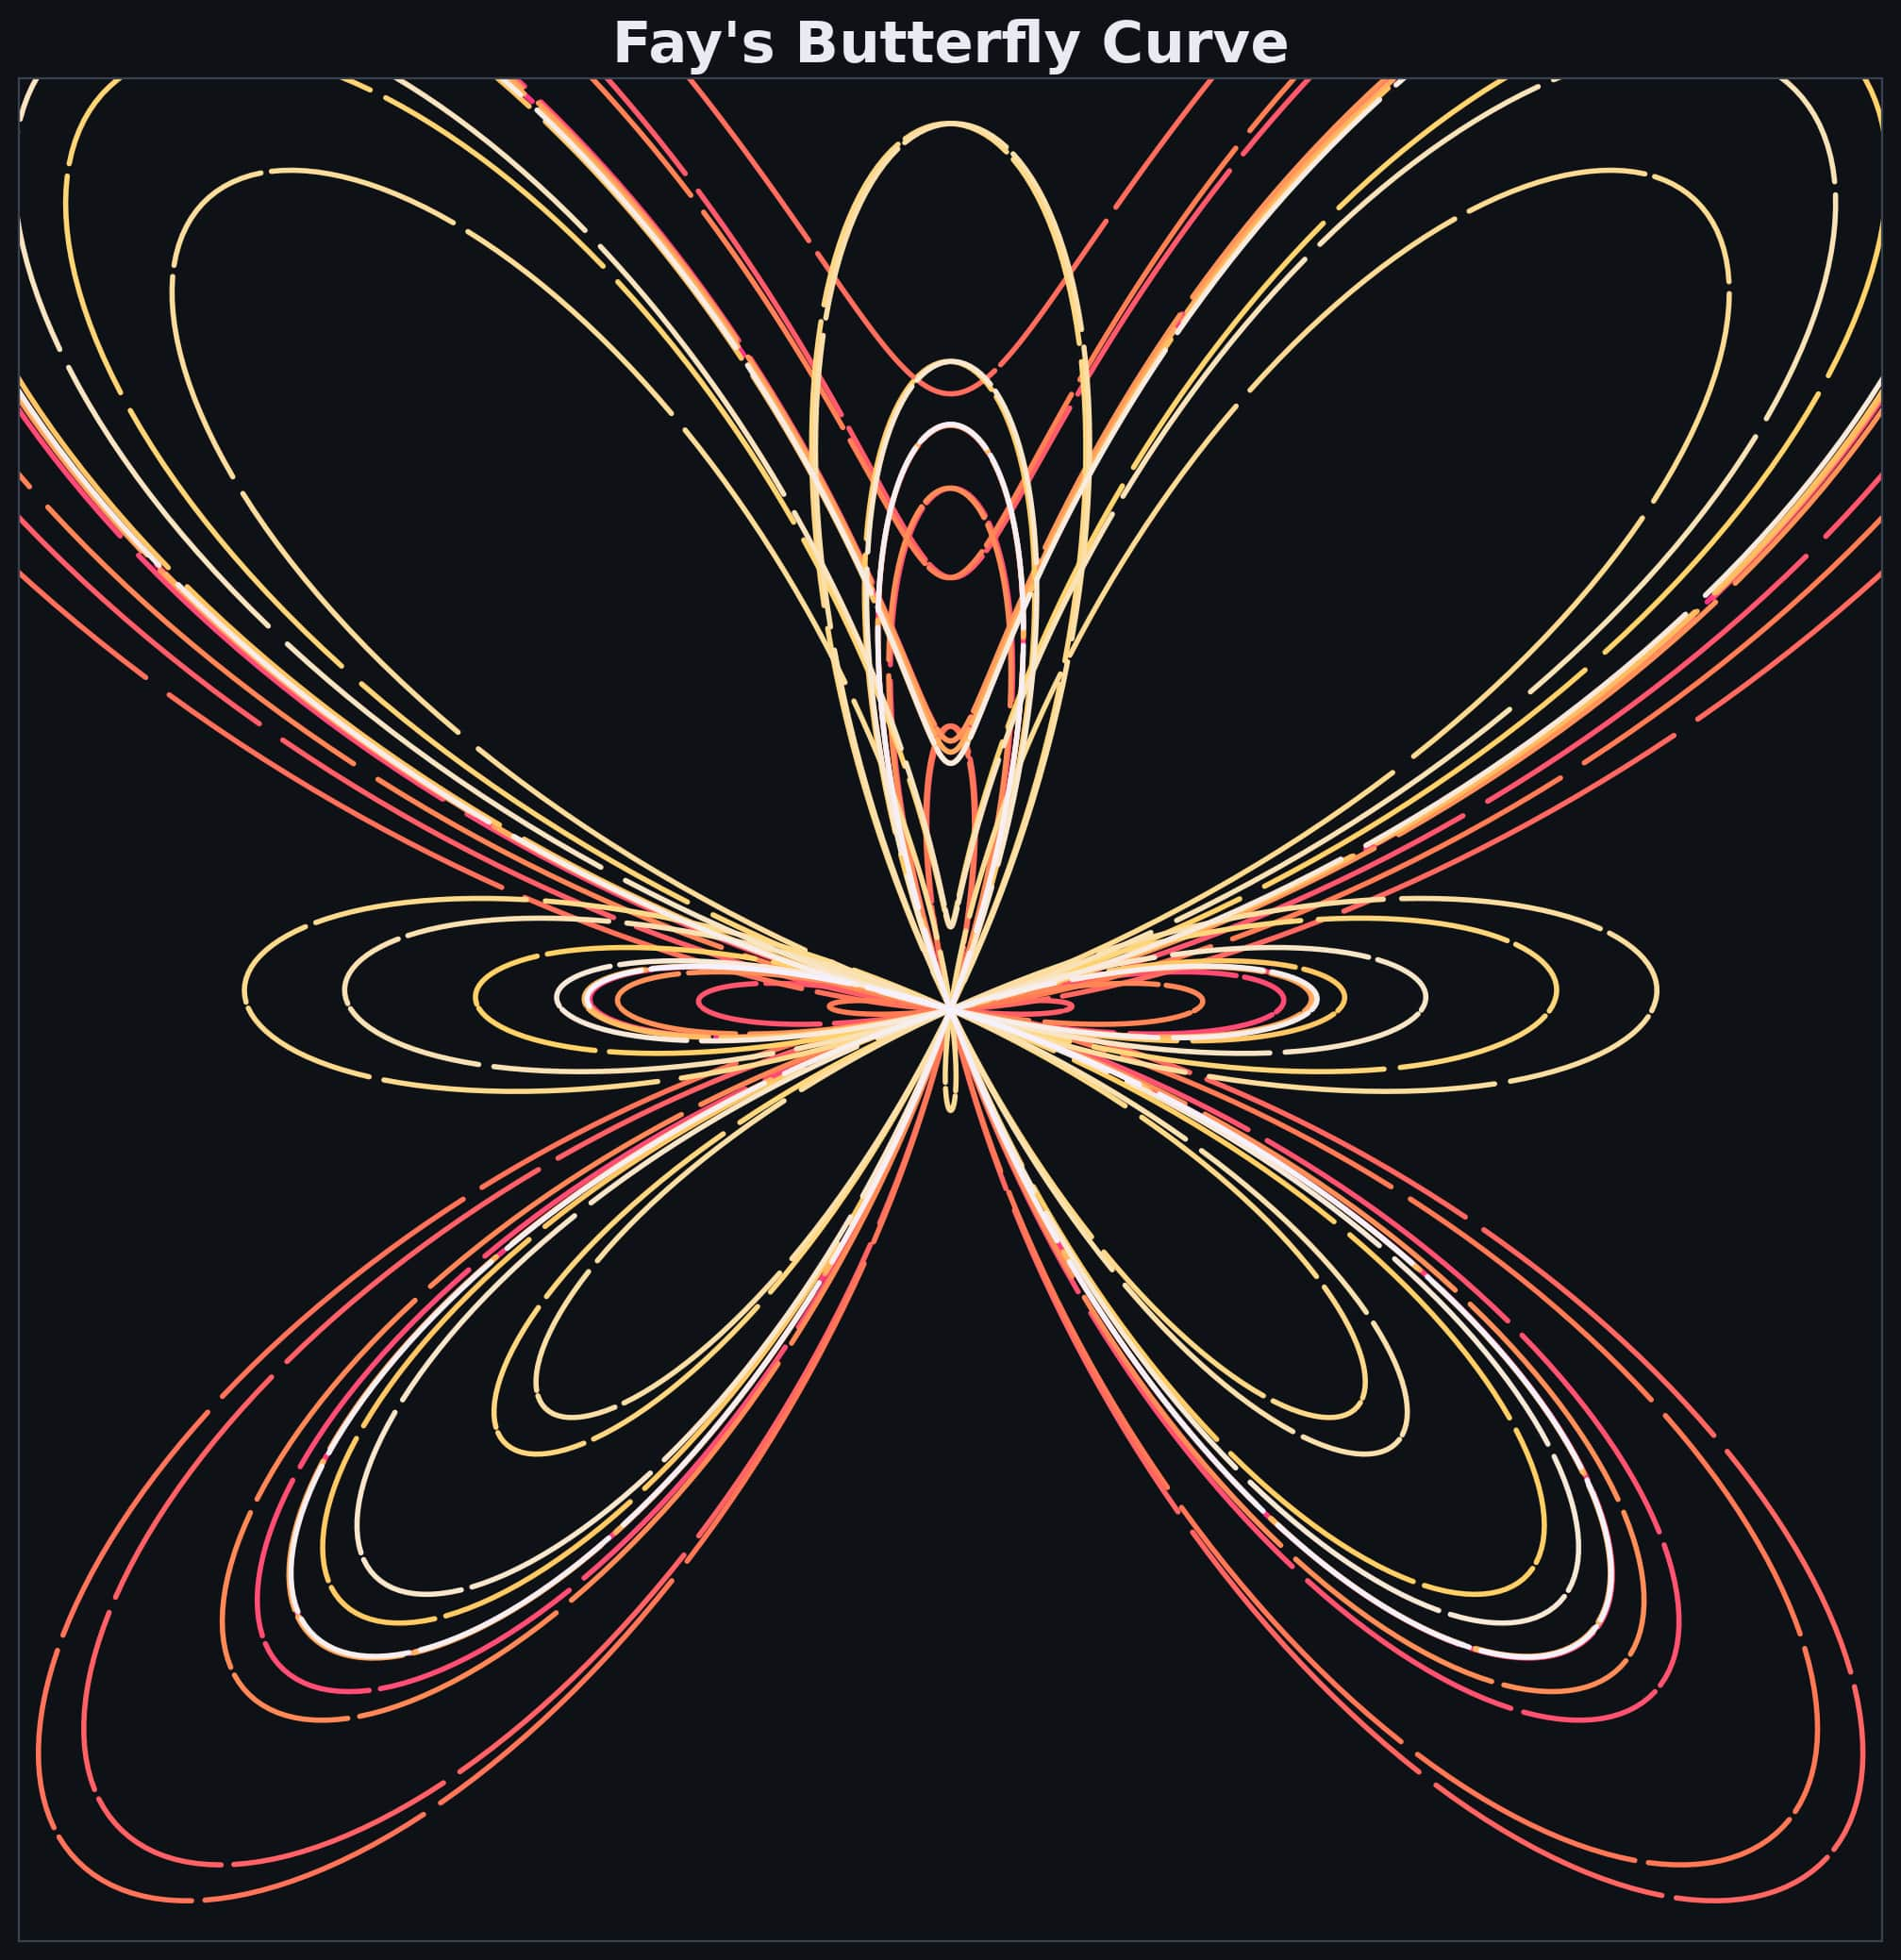
\includegraphics[width=\linewidth]{graphs/butterfly_curve}
		\caption{Fay's butterfly curve, \cref{butterfly}.}
		\label{fig:butterfly}
	\end{subfigure}
	\caption{Two families of closed parametric curves. (a) nine frequency
	ratios, each drawn at $\delta \in \{0, \pi/8, \pi/4\}$; the ratios are the
	ones tabulated in \cref{tab:ratios}. (b) twelve superimposed turns of
	\cref{butterfly}, coloured by $\theta$.}
	\label{fig:curves}
\end{figure}

Both figures were produced with the same routine: sample the parameter on a
uniform grid, evaluate, and plot the result as a single polyline. The only
thing that has to be chosen with care is the sample count. \Cref{butterfly}
needs roughly an order of magnitude more points than \cref{lissajous} to look
smooth, because its twelve turns cover twelve times the parameter range at
comparable curvature.

\newpage
